\section{Veje}
Vi har indtil videre snakket om kanter, og hvordan de enkeltvis er incidente med knudepar. I dette afsnit vil vi udvide det til at snakke om \emph{veje}, som er følger af disse kanter, og dermed er de også grafer i sig selv. Hvis der er tale om ikke-orienterede grafer, er veje defineret ved:
\begin{defn}
[Veje i ikke-orienterede grafer] 
Lad $n \in \N _0$  og $G$ være en ikke-orienteret graf. En vej, $P$, af længde $n$, fra $u$ til $v$, i $G$ er en følge af $n$ kanter,  $ P= (e_{1},e_{2},\dotsc,e_{n})$, for hvilken der eksisterer en følge, $u=x_{0}$ og $v=(x_{1},x_{2},\dotsc,x_{n-1}$,$x_{n})$, af knuder sådan at $e_{i}$ har, for $i=1,2,\dotsc,n$, endeknuderne $x_{i-1}$ og $x_{i}$. Når grafen er simpel, betegnes vejen ved grafens knudefølge, $x_{o},x_{1},\dotsc,x_{n}$. Hvis den ikke er simpel, beskrives vejen ved kanterne, $e_{1},e_{2},\dotsc,e_{n}$. 
\end{defn}
Her er en vej simpel, hvis den kun passerer den samme kant én gang. Kigger vi derimod på veje med orienterede grafer, som er det vi beskæftiger os med i problemet, ser definitionen en smule anderledes ud:
\begin{defn}
[Veje i orienterede grafer] 
Lad $n \in \N _0$ og $G$ være en orienteret graf. En vej, $P$, af længde $n$, fra $u = x_0$ til $v = x_n$, i $G$ er en følge af kanter, $e_{1},e_{2},\dotsc,e_{n}$, $ \exists (x_{n-1},x_{n}) $ for $e_{n} \forall e_n$. Hvis alle knudepar, i en given vej, højst har én kant som er incident med parret, betegner vi vejen ved dennes knudefølge $x_{o},x_{1},\dotsc,x_{n}$.
\end{defn}

\begin{figure}[H]
\centering
	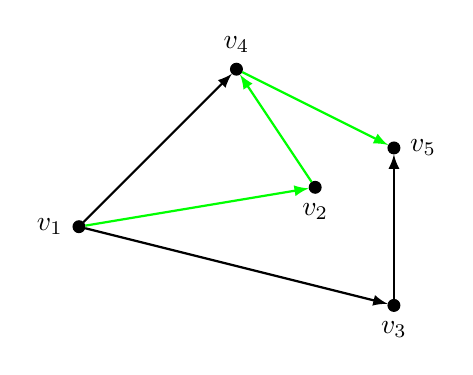
\begin{tikzpicture}

      \tikzset{enclosed/.style={draw, circle, inner sep=0pt, minimum size=.15cm, fill=black}}
%% Vertices
      	\node[enclosed, label={left: $v_1$}] (v1) at (0,2) {};
      	\node[enclosed, label={below: $v_2$}] (v2) at (3,2.5) {};
    		\node[enclosed, label={below: $v_3$}] (v3) at (4,1) {};
  	    \node[enclosed, label={above: $v_4$}] (v4) at (2,4) {};
     	\node[enclosed, label={right: $v_5$}] (v5) at (4,3) {};
%Edges
		\path [->, >=latex, thick, green](v1) edge node[midway, sloped, above] {} (v2);
		\path [->, >=latex, thick](v1) edge node[midway, sloped, above] {} (v3);
		\path [->, >=latex, thick](v1) edge node[midway, above] {} (v4);
		\path [->, >=latex, thick, green](v2) edge node[near end, sloped, below] {} (v4);
		\path [->, >=latex, thick](v3) edge node[midway, below] {} (v5);
		\path [->, >=latex, thick, green](v4) edge node[near end, sloped, above] {} (v5);

	\end{tikzpicture}
	\caption{Eksempel på en orienteret simpel graf og en vej fra $v_{0}$ til $v_{4}$}
	\label{fig.vaegtetopg}
\end{figure}

Antallet af veje mellem to knuder i grafen kan findes ved hjælp af nabomatricer, som vi diskuterede i forrige afsnit.
\begin{thm}
[Antallet af veje mellem to knuder] 
Lad G være en vilkårlig graf med nabomatricen
\textbf{$A$} med grafens knuder i rækkefølgen $v_{1},v_{2},\dotsc,v_{n}$. Antallet af forskellige veje med længde $r$ fra $v_{i}$ til $v_{j}$ vil da være lig den $(i,j)$'te indgang af \textbf{$A^{r}$}.
\end{thm}

\begin{proof}
Lad G være en graf med nabomatricen 
\textbf{$A$}, hvor vi antager, at knuderne i $G$ har rækkefølgen $v_{1},v_{2},\dotsc,v_{n}$. Antallet af veje fra $v_{i}$ til $v_{j}$ af længde 1 er da den $(i,j)$'te indgang til 
\textbf{$A$}. Dette skyldes, at det blot er antallet af kanter fra $v_{i}$ til $v_{j}$.
Vi antager, at den $(i,j)$'te indgang til 
\textbf{${A^r}$} er antallet af forskellige veje, som går fra $v_{i}$ til $v_{j}$ og som har længden $r$. Dette er hypotesen, vi ønsker at bekræfte.
Vi ser på nabomatricen \textbf{$A^{r+1}$}. 
\textbf{$A^{r+1}$} er det samme som 
\textbf{$A^{r}$}$\cdot$\textbf{$A$}. Derfor må indgangen til \textbf{$A^{r+1}$} være produktet af indgangene til \textbf{$A^{r}$} og kanterne fra \textbf{$A^{r}$} til \textbf{$A^{r+1}$}. Vi siger, at $b_{ik}$ er den $(i,k)$'te indgang til 
\textbf{$A^{r}$}, som ifølge vores hypotese er antallet af veje fra $v_{i}$ til $v_{k}$ med længde $r$. Vi siger også at $a_{k,j}$ er den $(k,j)$'te indgang til 
\textbf{$A^{r+1}$}, som ifølge vores hypotese er antallet af veje fra $v_{k}$ til $v_{j}$ med længde $1$, hvilket vil sige kanterne mellem punkterne. Derved får vi den $(i,j)$'te indgang af \textbf{$A^{r+1}$} til at være: 

\begin{equation}
A^{r+1}=b_{i1}a_{1j} + b_{i2}a_{2j} +\dotsc+ b_{in}a_{nj}
\end{equation}

Det ses altså, at en vej af længde $r + 1$ fra $v_{i}$ til $v_{j}$ er lavet ud fra en vej med længden $r$ fra begyndelsesknuden $v_{i}$ og hen til en mellemliggende knude $v_{k}$ samt den kant, der går fra $v_{k}$ til $v_{j}$. 
Da dette er summen af produktet af alle veje med længden r fra $v_{i}$ til $v_{k}$ og alle kanter fra $v_{k}$ til $v_{j}$, som har længden 1, og dette findes for alle mulige $v_{k}$ kan ovenstående ligning også omskrives til: 

\begin{equation}
A^{r+1}=\sum_{k=1}^{K} b_{ik} a_{kj}
\end{equation}

For den første mulige $v_{k}$ har vi altså $b_{i1}$, som er antallet af veje fra $v_{i}$ til den første $v_{k}$, og $a_{1j}$ er vejen fra den første $v_{k}$ til $v_{j}$. Det ses, at produktet af disse to lægges sammen med produktet for de resterende $v_{k}$, så vi har antallet af alle mulige veje fra $v_{i}$ til $v_{j}$ gennem alle mulige $v_{k}$. Antallet af veje fra $v_{i}$ til $v_{j}$ med længde $r+1$ vil da være den (i,j)'te indgang til $A^{r+1}$. Derfor må det også gælde, at antallet af veje fra $v_{i}$ til $v_{j}$ med længde $r$ vil være den (i,j)'te indgang til $A^{r}$, hvilket var det, vi ville bevise.

\end{proof}

\begin{exmp}
Vi starter med at kigge på en graf og den tilhørende nabomatrix:
\begin{figure}[H]
\centering
	\begin{tikzpicture}

      \tikzset{enclosed/.style={draw, circle, inner sep=0pt, minimum size=.15cm, fill=black}}
%% Vertices
      	\node[enclosed, label={left: $v_1$}] (v1) at (1,2) {};
      	\node[enclosed, label={above: $v_2$}] (v2) at (3,4) {};
    	\node[enclosed, label={below: $v_3$}] (v3) at (1,0) {};
  	    \node[enclosed, label={right: $v_4$}] (v4) at (5,2) {};
     	\node[enclosed, label={below: $v_5$}] (v5) at (5,0) {};
%Edges
		\path (v1) edge node[midway, sloped, above] {} (v2);
		\path (v1) edge node[midway, sloped, above] {} (v3);
		\path (v1) edge node[midway, above] {} (v4);
		\path (v2) edge node[near end, sloped, below] {} (v4);
		\path (v3) edge node[midway, below] {} (v5);
		\path (v4) edge node[near end, sloped, above] {} (v5);

	\end{tikzpicture}
	\caption{Eksempel på en ikke-orienteret simpel graf}
	\label{fig.vaegtetopg}
\end{figure}

\begin{equation}
A=\begin{bmatrix}
    0&1&1&1&0\\
    1&0&0&1&0\\
    1&0&0&0&1\\
    1&1&0&0&1\\
    0&0&1&1&0\\
\end{bmatrix}
\end{equation}


Vi ønsker at finde ud af hvor mange veje med en længde på 4, der går fra $v_1$ til $v_5$. Det ses i nabomatricen, at $v_1$ har 3 naboer, nemlig $v_2$, $v_3$ og $v_4$. Fortsætter vi, kan vi se, at $v_2$ har $v_1$ og $v_4$ som naboer, $v_3$ har $v_1$ og $v_5$, og $v_4$ har $v_1$, $v_2$ og $v_5$ som naboer. Fortsætter vi, så vi finder alle tænkelige veje med længder på 3, får vi, at der er 18 forskellige veje, der alle starter i $v_1$ og har en længde på 3. Vi skal nu finde de veje, der ved at tilføje en kant, ender i $v_5$. Vi kan se, at $v_5$ har $v_3$ og $v_4$ som naboer. Vi finder derfor de veje, der starter i $v_1$ og slutter i $v_3$, med længden 3, og derefter dem, der slutter i $v_4$, med længden 3. På denne måde udnytter vi, hvad vi skrev i beviset, nemlig at
\textbf{$A^{r+1}$} er lig med $b_{i1}a_{1j} + b_{i2}a_{2j} +\dotsb+ b_{in}a_{nj}$
Her er $b_{ik}$ antallet af veje fra $v_{i}$ til ${v_k}$. I vores eksempel er $v_{i}=v_{1}$, ${v_{k1}}=v_{3}$, ${v_{k2}}=v_{4}$, $v_{j}=v_{5}$ og \textbf{$A^{r+1}$}=\textbf{$A^{3+1}$}. 
 
\begin{figure}[H]
\centering
	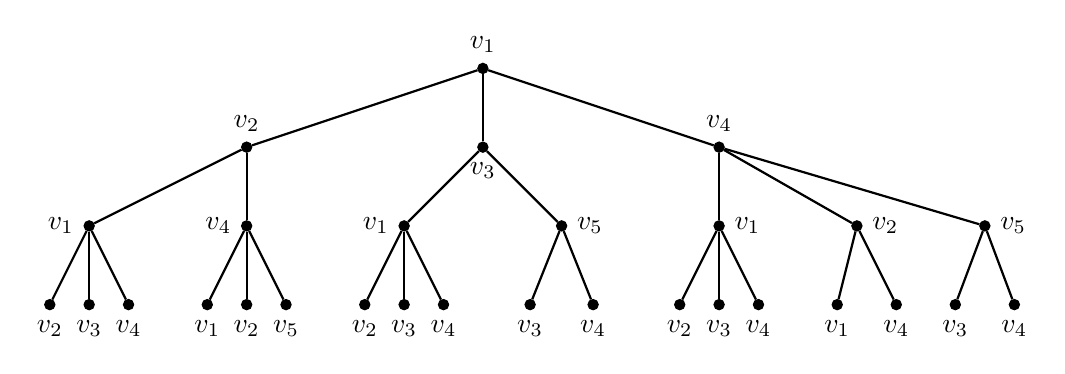
\begin{tikzpicture}

      \tikzset{enclosed/.style={draw, circle, inner sep=0pt, minimum size=.13cm, fill=black}}
%% Vertices
      	\node[enclosed, label={above: $v_1$}] (v1) at (3,6) {};
      	\node[enclosed, label={above: $v_2$}] (v2) at (0,5) {};
    		\node[enclosed, label={below: $v_3$}] (v3) at (3,5) {};
  	    \node[enclosed, label={above: $v_4$}] (v4) at (6,5) {};
     	\node[enclosed, label={left: $v_1$}] (v5) at (-2,4) {};
     	\node[enclosed, label={left: $v_4$}] (v6) at (0,4) {};
     	\node[enclosed, label={left: $v_1$}] (v7) at (2,4) {};
     	\node[enclosed, label={right: $v_5$}] (v8) at (4,4) {};
     	\node[enclosed, label={right: $v_1$}] (v9) at (6,4) {};
     	\node[enclosed, label={right: $v_2$}] (v10) at (7.75,4) {};
     	\node[enclosed, label={right: $v_5$}] (v11) at (9.375,4) {};
     	\node[enclosed, label={below: $v_2$}] (v12) at (-2.5,3) {};
      	\node[enclosed, label={below: $v_3$}] (v13) at (-2,3) {};
  	    \node[enclosed, label={below: $v_4$}] (v14) at (-1.5,3) {};
  	    \node[enclosed, label={below: $v_1$}] (v15) at (-0.5,3) {};
     	\node[enclosed, label={below: $v_2$}] (v16) at (0,3) {};
     	\node[enclosed, label={below: $v_5$}] (v17) at (0.5,3) {};
     	\node[enclosed, label={below: $v_2$}] (v18) at (1.5,3) {};
      	\node[enclosed, label={below: $v_3$}] (v19) at (2,3) {};
  	    \node[enclosed, label={below: $v_4$}] (v20) at (2.5,3) {};
  	    \node[enclosed, label={below: $v_3$}] (v21) at (3.6,3) {};
  	    \node[enclosed, label={below: $v_4$}] (v22) at (4.4,3) {};
  	    \node[enclosed, label={below: $v_2$}] (v23) at (5.5,3) {};
      	\node[enclosed, label={below: $v_3$}] (v24) at (6,3) {};
  	    \node[enclosed, label={below: $v_4$}] (v25) at (6.5,3) {};
  	    \node[enclosed, label={below: $v_1$}] (v26) at (7.5,3) {};
     	\node[enclosed, label={below: $v_4$}] (v27) at (8.25,3) {};
     	\node[enclosed, label={below: $v_3$}] (v28) at (9,3) {};
     	\node[enclosed, label={below: $v_4$}] (v29) at (9.75,3) {};
%Edges
		\path[thick] (v1) edge node[midway, sloped, above] {} (v2);
		\path[thick] (v1) edge node[midway, sloped, above] {} (v3);
		\path[thick] (v1) edge node[midway, above] {} (v4);
		\path[thick] (v2) edge node[near end, sloped, below] {} (v5);
		\path[thick] (v2) edge node[midway, below] {} (v6);
		\path[thick] (v3) edge node[near end, sloped, above] {} (v7);
		\path[thick] (v3) edge node[near end, sloped, above] {} (v8);
		\path[thick] (v4) edge node[near end, sloped, above] {} (v9);
		\path[thick] (v4) edge node[near end, sloped, above] {} (v10);
		\path[thick] (v4) edge node[near end, sloped, above] {} (v11);
		\path[thick] (v5) edge node[near end, sloped, above] {} (v12);
		\path[thick] (v5) edge node[near end, sloped, above] {} (v13);
		\path[thick] (v5) edge node[near end, sloped, above] {} (v14);
		\path[thick] (v6) edge node[near end, sloped, above] {} (v15);
		\path[thick] (v6) edge node[near end, sloped, above] {} (v16);
		\path[thick] (v6) edge node[near end, sloped, above] {} (v17);
		\path[thick] (v7) edge node[near end, sloped, above] {} (v18);
		\path[thick] (v7) edge node[near end, sloped, above] {} (v19);
		\path[thick] (v7) edge node[near end, sloped, above] {} (v20);
		\path[thick] (v8) edge node[near end, sloped, above] {} (v21);
		\path[thick] (v8) edge node[near end, sloped, above] {} (v22);
		\path[thick] (v9) edge node[near end, sloped, above] {} (v23);
		\path[thick] (v9) edge node[near end, sloped, above] {} (v24);
		\path[thick] (v9) edge node[near end, sloped, above] {} (v25);
		\path[thick] (v10) edge node[near end, sloped, above] {} (v26);
		\path[thick] (v10) edge node[near end, sloped, above] {} (v27);
		\path[thick] (v11) edge node[near end, sloped, above] {} (v28);
		\path[thick] (v11) edge node[near end, sloped, above] {} (v29);

	\end{tikzpicture}
	\caption{De mulige løsninger for veje med længde 3 fra $v_{0}$ til $v_{k}$.}
	\label{fig.vaegtetopg}
\end{figure}

Antallet af veje fra $v_{1}$ til $v_{3}$ er 5, og antallet af veje fra $v_{1}$ til $v_{4}$ er 6. Vi kan derfor opstille
\textbf{$A^{4}$}$=b_{i1} a_{1j}+b_{i2} a_{2j}=5 \cdot 1+6 \cdot 1=11$.
Her er $b_{i1}$ antallet af veje fra $v_{1}$ til $v_{3}$, og $a_{1j}$ er antallet af kanter fra $v_{3}$ til  $v_{5}$. På samme måde optræder $b_{i2}$ og $a_{2j}$ for $v_{4}$. Der er altså 11 veje med længden 4 fra $v_{1}$ til $v_{5}$.

\end{exmp}

\input{incl/main/grafer/vægtede}